%!TEX TS-program = xelatex
\documentclass[a4paper, 12pt]{article}
\usepackage{barinovxesimple}
\geometry{top=25mm}
\geometry{bottom=35mm}
\geometry{left=35mm}
\geometry{right=20mm}
\setlist{labelindent=\parindent,leftmargin=*}
\begin{document}
\thispagestyle{empty}
\begin{center}
    \textit{Федеральное государственное автономное образовательное\\ учреждение высшего образования }

    \vspace{0.5ex}

        \textbf{«Московский физико-технический институт\\ (национальный исследовательский университет)»}
\end{center}

\vspace{10ex}

\begin{center}
    \vspace{13ex}

    \so{\textbf{Лабораторная работа №-.-.-}}

    \vspace{1ex}

    по курсу общей физики

    на тему:

    \textbf{\textit{<<>>}}

    \vspace{30ex}

    \begin{flushright}
        \noindent
        \textit{Работу выполнил:}\\  
        \textit{Баринов Леонид \\(группа Б02-827)}
    \end{flushright}
    \vfill
    Долгопрудный \\2019
\newpage
\setcounter{page}{1}
\fancyhead[R]{\nouppercase{\leftmark}}	
\end{center}


\section{Цель работы}
Исследовать электронный парамагнитный резонанс в молекуле ДФПГ, определить $g$-фактор
электрона, измерить ширину линии электронного парамагнитного резонанса
(ЭПР).


\section{Суть исследуемого явления}
Суть явления электронного парамагнитного резонанса заключается в
резонансном поглощении электромагнитного излучения неспаренными
электронами за счет возбуждения электронных резонансных переходов
(имеющих частоту, определяемую формулой \eqref{eq:3})
электромагнитным полем.



\section{Теория явления}
Атомы и молекулы, имеющие незаполненную электронную оболочку, обладают
электронными магнитными моментами $\vec{\mu}$ даже в отсутствии
внешнего магнитного поля. Особенно явно эти свойства выражены у
свободных радикалов, а также у многих $d$−элементов. Во внешнем
магнитном поле $\vec{H}_{0}$ магнитные дипольные моменты частиц
стремятся выстроиться вдоль поля, поскольку такое положение
минимизирует их энергию:
\begin{equation}
    E = -(\vec{\mu}, \vec{H}_{0})
    \label{eq:1}
\end{equation}

\begin{wrapfigure}{r}{0.46\linewidth}
    \includegraphics{1}
    \caption{Энергетические уровни электрона во внешнем магнитном
    поле $\vec{H}_{0}$}
    \label{fig:1}
\end{wrapfigure}

Магнитный момент частицы связан с ее механическим моментом $\vec{J}$
гиромагнитным отношением: $\vec{\mu}=\gamma \vec{J}$. Обе эти величины
квантуются:
\begin{equation*}
    \begin{gathered}
        J_z = m_J \hbar, \hspace{1em} mJ = -J, -J+1, \ldots, J\\
        \mu_z = \gamma \hbar m_J = -g \mu_\text{Б} m_J
    \end{gathered}
\end{equation*}
где $\mu_\text{Б} = e \hbar / 2mc$ --- величина размерности магнитного
момента, называемая магнетоном Бора. Во внешнем магнитном поле уровни
энергии парамагнитной частицы расщепляются на дискретные подуровни:
\begin{equation}
    E = - (\vec{\mu}, \vec{H}_{0}) = g \mu_\text{Б} H_0 m_J
    \label{eq:2}
\end{equation}



Под действием электромагнитного излучения будут происходить переходы
между такими уровнями, если энергия кванта излучения близка к разнице
энергий между ними и соблюдается правило отбора по магнитному
квантовому числу $\Delta m_J = \pm 1$:
\begin{equation}
    \hbar \omega = \Delta E = h \mu_\text{Б} H_0
    \label{eq:3}
\end{equation}


Поскольку в стационарном состоянии на более низком энергетическом
уровне находится больше частиц, а вероятности переходов одинаковы, то
в итоге будут преобладать переходы снизу вверх, т.е. с поглощением
излучения. Такое избирательное поглощение энергии системой
парамагнитных частиц при определенном отношении напряженности
постоянного магнитного поля к частоте радиоизлучения и получило
название электронного парамагнитного резонанса.

Стоит отметить неоспоримое достоинство данного метода по сравнению с
другими спектральными методами, заключающееся в
том, что мы можем сами устанавливать расстояние между энергетическими
уровнями, изменяя внешнее магнитное поле. При этом характеристики
поглощаемого веществом ЭМ-поля могут быть оставлены без изменения.




\section{Эксперимент}
\subsection{Экспериментальная установка}
В данной работе используется радиоспектроскоп, работающий в диапазоне
100 ÷ 200 МГц. Его действие основано на уменьшении добротности
контура при появлении резонансных парамагнитных потерь. Схема
радиоспектроскопа изображена на \fig{fig:2}. Основной частью
радиоспектроскопа является колебательный контур. Он состоит из
катушки индуктивности и плоского конденсатора. Контур заключён в
латунный посеребренный изнутри контейнер. Ампула с исследуемым
образцом (ДФПГ) вставляется в катушку индуктивности контура. Основное
магнитное поле в образце создаётся с помощью двух соосно расположенных
катушек, питаемых от источника постоянного тока. Величина тока,
протекающего через катушки, регулируется ручкой, расположенной на
блоке питания, и измеряется при помощи вольтметра и омического
сопротивления $R$, включённого последовательно с катушками.

\begin{wrapfigure}{l}{0.5\linewidth}
    \includegraphics[width=\linewidth]{2}
    \caption{Блок-схема установки для наблюдения ЭПР}
    \label{fig:2}
\end{wrapfigure}

Небольшое модулирующее поле создаётся при помощи дополнительных
катушек. Они включены в сеть переменного тока через трансформатор.
Общая ось основных и дополнительных катушек перпендикуляр- на оси
катушки индуктивности контура.

Электромагнитные колебания в контуре возбуждаются генератором
радиочастотного диапазона. Связь с генератором осуществляется с
помощью петли. Через полупроводниковый диод контур подключён к
вертикальному усилителю осциллографа. Колебательный контур соединён с
генератором и осциллографом коаксиальным кабелем.

Величина постоянного магнитного поля $H$, резонансная частота
колебательного контура и частота генератора $\omega$ выбираются так, чтобы
они были близки к значениям, удовлетворяющим условию \eqref{eq:5}. Небольшое
переменное магнитное поле катушек модулирует основное магнитное поле
и два раза за каждый период заставляет его проходить через точное
резонансное значение $H_0$ (при данной частоте $\omega$).

При наступлении электронного парамагнитного резонанса поглощение
энергии в образце увеличивается, добротность колебательного контура
падает, и амплитуда колебаний в контуре уменьшается. В зависимости
от полярности диода пик сигнала электронного парамагнитного
резонанса на экране осциллографа обращён вверх или вниз от
горизонтальной линии развёртки.

Величина постоянного поля измеряется следующим образом.
Сначала режим подачи тока на основные катушки изменяется с
постоянного на переменный. Ток подбирается таким образом, чтобы
показания вольтметра, подключенного к резистору $R$ (см. \fig{fig:2})
соответствовало показаниям до смены режима. Далее внутрь основных
катушек поблизости от образца вводится пробная катушка и измеряются
показание лампового милливольтметра $V$. Зная число витков $n$ и площадь
сечения $S$ пробной катушки (эти величины указаны на ней), а также
частоту подаваемого на модулирующие катушки сигнала $\omega _{\sim} =
2\pi \cdot 50\: \text{Гц}$,
можно определить величину магнитного поля $H_0$ из соотношения
\begin{equation}
    V = n H_0 S \omega _{\sim}.
    \label{eq:4}
\end{equation}

Конечная формула зависимости частоты сигнала генератора от показаний
лампового вольтметра $\nu(V)$
\begin{equation}
    \nu = \frac{g \nu _{\text{Б}}}{\pi^3 d^2 n \hbar \nu _{\sim}}V
    \label{eq:5}
\end{equation}



\section{Результаты эксперимента}
В результате настройки силы тока в катушках при значении частоты
генератора $\nu = 162\: \text{МГц}$ на осциллографе была получена характерная для
резонанса картина. Форма линии поглощения при подаче на X–канал
сигнала с модуляционных катушек представлена на \fig{fig:3}.



\begin{figure}[H]
    \includegraphics[width=0.5\linewidth]{3} 
    \caption{Форма линии поглощения}
    \label{fig:3}
\end{figure}




\begin{figure}[H]
    \floatsetup{heightadjust=object,valign=c}
    \begin{floatrow}

        \ffigbox{
        \caption{Осциллограмма сигнала поглощения при подаче переменного тока в
        основную катушку. Амплитуда достигла 
        резонансного значения}
    }
        {
        \includegraphics[width=0.7\linewidth]{5}
        \label{fig:4}
    }

        \ffigbox{
        \caption{Осциллограмма сигнала поглощения при подаче переменного тока в
        основную катушку. Амплитуда переменного поля превысила
    резонансное значение, пики раздвоились}
    }
        {
        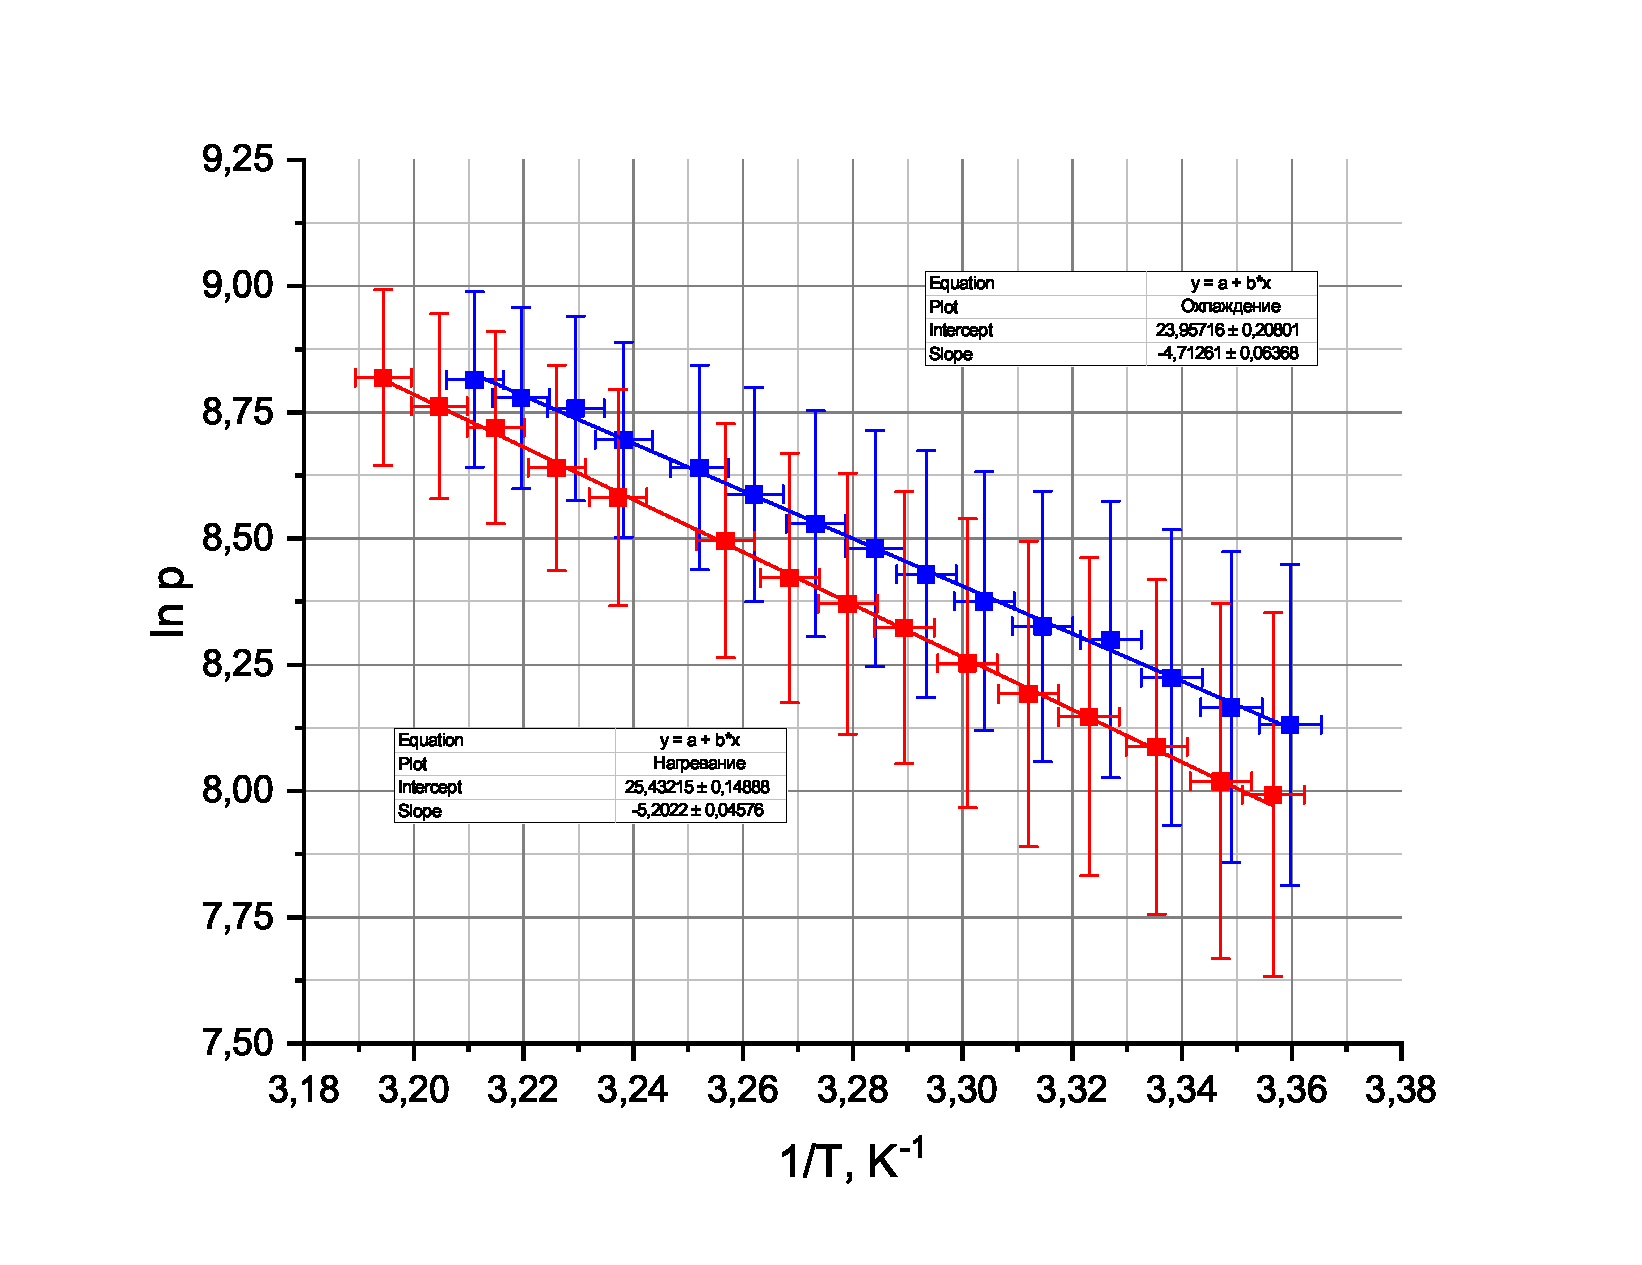
\includegraphics[width=0.7\linewidth]{4}
        \label{fig:5}
    }
    \end{floatrow}
\end{figure}









\section{Анализ результатов}
Моделирующие поле может быть рассчитано по формуле, в которой $d = 15,2\:
\text{мм}$, $n = 45$:
\begin{equation}
    B _{\text{мод}} = \sqrt{2} \frac{2 V_\text{мод}}{\pi^2 d^2 n
    \nu_\sim}
    \label{eq:6}
\end{equation}

Ширина спектральной линии теперь может быть
оценена как 
\begin{equation}
    \Delta B = B_\text{мод} \cdot \frac{l}{L}
    \label{eq:7}
\end{equation}

Вычислим значение $\Delta B$, взяв $l = 0,6$, $L = 6,8$, определенные
по осциллограмме на \fig{fig:3}.
\[
    \Delta B = (1,7 \pm 0,3)\: \text{Гс}
\]


При значении частоты сигнала генератора $\nu = 161,5\: \text{МГц}$
был подобран соответствующий резонансный 
ток, после чего 
было измерено напряжение на пробной катушке. Определим $g$ по формуле
\eqref{eq:5}:
\[
    g = 2,04 \pm 0,03
\]







\section{Выводы}
В данной работе был изучен метод электронного парамагнитного
резонанса, с помощью которого был найден $g$-фактор электрона, а также
была получена ширина спектральной линии ДФПГ:
\begin{equation*}
    \begin{gathered}
    \Delta B = (1,7 \pm 0,3)\: \text{Гс}\\
    g = 2,04 \pm 0,03
    \end{gathered}
\end{equation*}
Оба результата находятся
в соответствии с табличными значениями.
\begin{equation*}
    \begin{gathered}
    \Delta B^\text{т} = 2\: \text{Гс}\\
    g^\text{т} = 2
    \end{gathered}
\end{equation*}









\end{document}
